\begin{enumerate}[label=\thesection.\arabic*.,ref=\thesection.\theenumi]
\numberwithin{equation}{enumi}

\item

For a control system in unity feedback with a transfer function
\begin{align}
    G(s) = \frac{10K}{s(s+1)(s+5)}
\end{align}
Design a lead compensator with a $60^{\degree}$ phase margin and an appropriate error constant of 5

\item
\solution
Before adding a compensator, we first find a value of gain for an error constant of 5. As the system has one pole at the origin, the appropriate error constant would be the velocity constant $K_{v}$. For an error constant of 5, we solve the following equation:
\begin{align}
    \lim_{s \to 0} s G(s) = \lim_{s \to 0} \frac{10K}{(s+1)(s+5)} = 2K\\
    \implies K = \frac{K_{v}}{2} = 2.5
\end{align}
So, the new transfer function becomes
\begin{align}
    G(s) = \frac{25}{s(s+1)(s+5)}
\end{align}
The gain crossover frequency $ \omega_{gc} $ and phase margin $ \phi_{M} $ is calculated from the plots using the following code
\begin{lstlisting}
codes/ee18btech11051/ee18btech11051_code1.py
\end{lstlisting}

\begin{figure}[!ht]
    \centering
    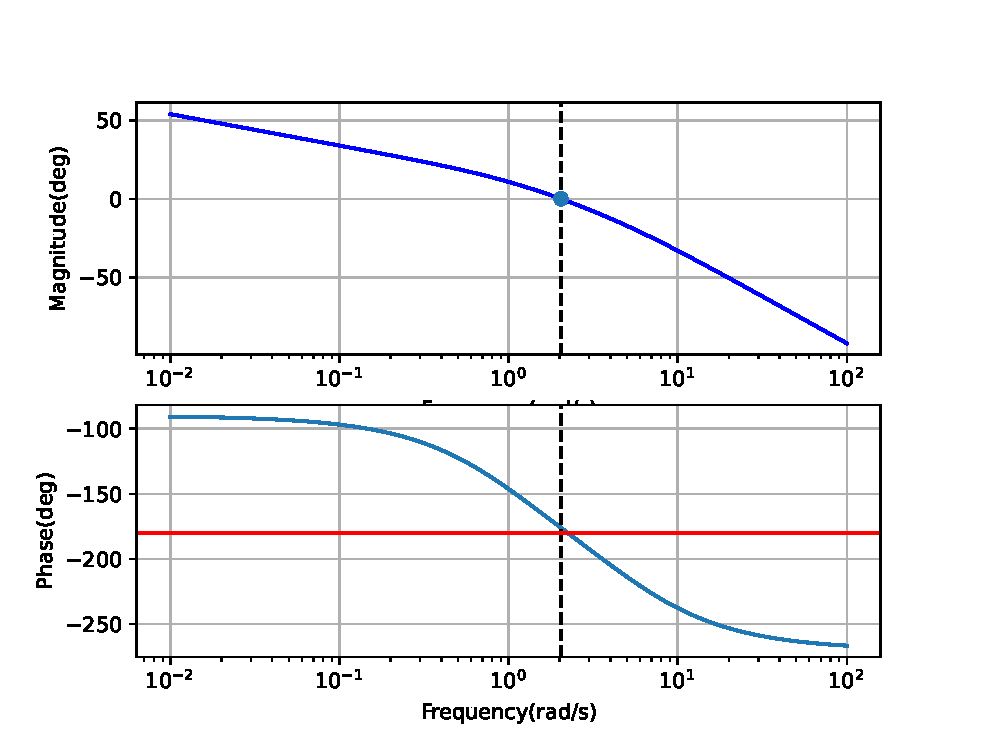
\includegraphics[width=\columnwidth]{./figs/ee18btech11051/ee18btech11051_fig1.eps}
    \label{fig:ee18btech11051_1}
\end{figure}

This can also be calculated from the equations
\begin{align}
    \omega \sqrt{\omega^2 + 1} \sqrt{\omega^2 + 25} = 25\\
    \phi_{M} = -90^{\circ} - \tan^{-1}{\omega_{gc}} - \tan^{-1}({\frac{\omega_{gc}}{10}})
\end{align}

Solving which, we get $\phi_{M} =  3.96^{\degree} , \omega_{gc} =  2.03$\\
The following code computes the margins and frequencies:
\begin{lstlisting}
codes/ee18btech11051/ee18btech11051_code2.py
\end{lstlisting}

The maximum phase of the compensator is given by-
\begin{align}
    \phi_{M} = 60^{\degree} - phase margin + angle correction\\
    \phi_{M} = 56^{\degree} + angle correction
\end{align}
Here, the angle correction is added to compensate the early zero added due to the lead compensator. The highest phase margin is achieved when $\phi_{M}$ is close to $90^{\degree}$. To achieve it, we take angle correction = $33^{\degree}$.
The phase lead compensator will have a transfer function of the form:
\begin{align}
    G_{C}(s) = \left(\frac{1+\alpha Ts} {1+Ts}\right), \alpha >1
\end{align}


Note that this transfer function doesn't change the error constant.
Now we solve for $\alpha$ using the equation
\begin{align}
    \alpha = \frac{1+\sin{\phi_{M}}}{1-\sin{\phi_{M}}} = \frac{1+\sin{89^{\degree}}}{1-\sin{89^{\degree}}} = 13,130.56
\end{align}

Now to get the phase gain, we set the frequency for maximum phase of compensator $\omega_{m}$ to the previous gain crossover frequency. And using it, the value of T is calculated as follows
\begin{align}
    \omega_{m} = 2.03 rad/sec \\
    T = \frac{1}{\omega_{m}\alpha} = 0.0000375
\end{align}


The Compensator will have the transfer function as follows :
\begin{align}
G_{c}(s) = \left(\frac{1 + 0.5s}{1 + 0.0000375s}\right)
\end{align}

The open loop T.F for the compensated system is  :
\begin{align}
    G(s) G_{c}(s) = 25\left(\frac{(1+0.5s)}{s(s+1)(s+5)(1+0.0000375s)}\right)
\end{align}


To observe the changes, we plot the compensated system

\begin{figure}[!ht]
    \centering
    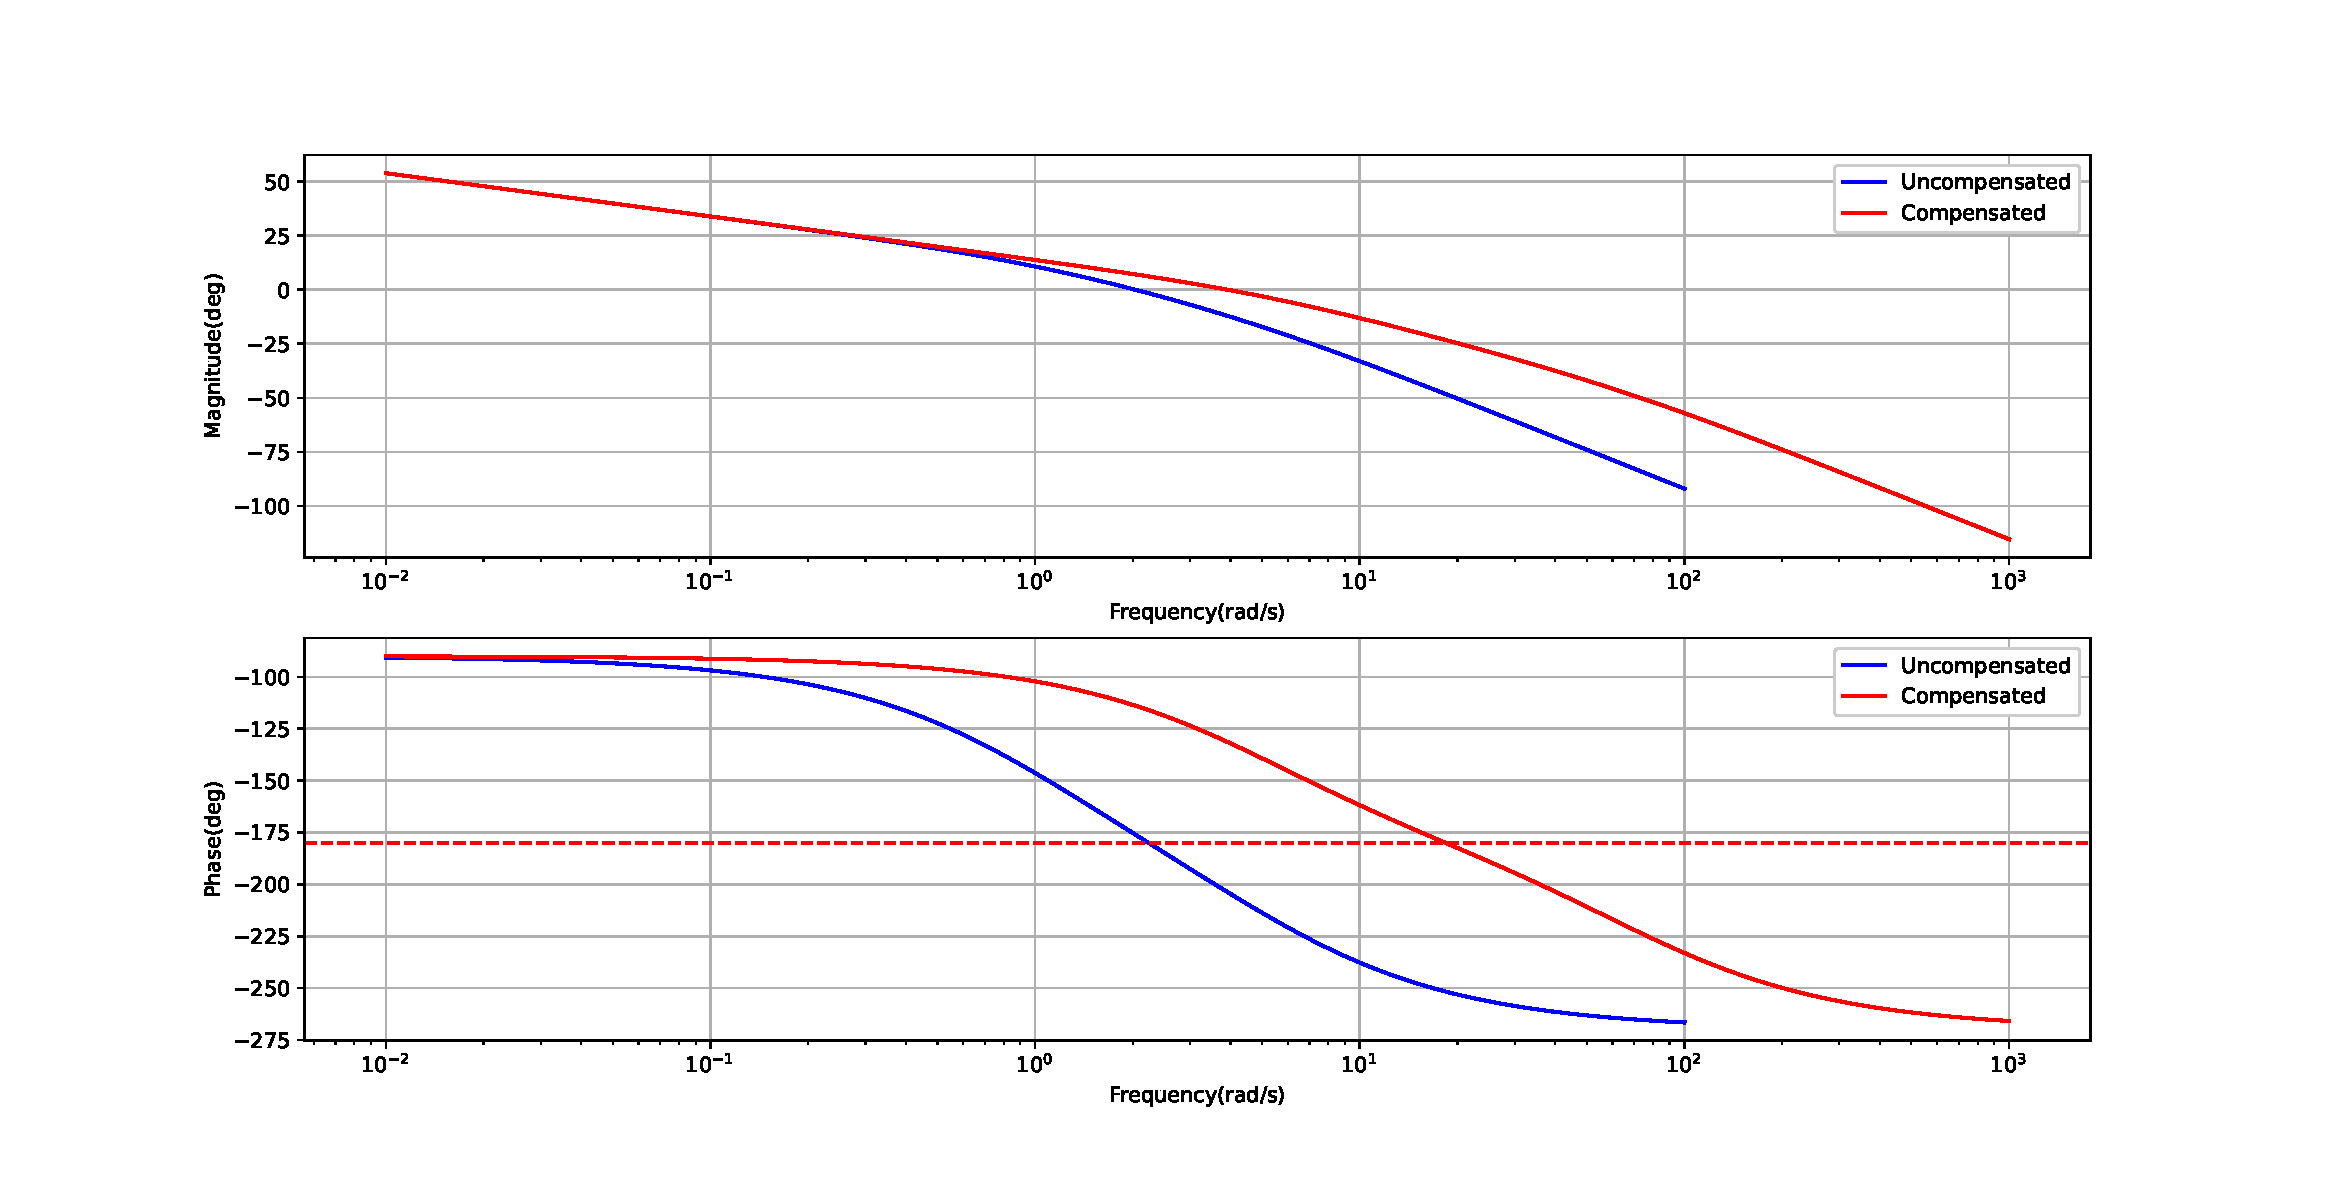
\includegraphics[width=\columnwidth]{./figs/ee18btech11051/ee18btech11051_fig2.eps}
    \label{fig:ee18btech11051_2}
\end{figure}

Using the code previously used to calculate the phase margin, the phase margin of the compensated system turns out to not go beyond $46^{\degree}$. So, we use a two stage lead compensator to get the required phase margin. The new compensator can be thought of as the square of the previous compensator 
\begin{align}
    G_{C}^{2}(s) = \left(\frac{1+\alpha Ts} {1+Ts}\right)^{2}, \alpha >1
\end{align}
The values of $\alpha$ and T can still be calculated as done previously, but for half of the required increase in phase, as the compensator gives double of the configured phase. So, for
\begin{align}
    \phi_{M} = \frac{(56^{\degree}+26^{\degree})}{2} = 41^{\degree}\\
    \alpha = \frac{1+\sin(38^{\degree})}{1-\sin{38^{\degree}}} = 5\\
    \omega_{m} = 2.6\\
    T = \frac{1}{\omega_{m}\alpha} = 0.0769
\end{align}
Now, the new compensator and the compensated transfer functions are
\begin{align}
    G_{c}^{2}(s) = \frac{(1 + 0.38s)^{2}}{(1 + 0.0769s)^{2}}\\
    G(s) G_{c}^{2}(s) = 25\left(\frac{(1+0.38s)^{2}}{s(s+1)(s+5)(1+0.0769s)^{2}}\right)
\end{align}


\item
\textbf{Verification : }
Now we plot the newly compensated transfer function.\\

\begin{figure}[!ht]
    \centering
    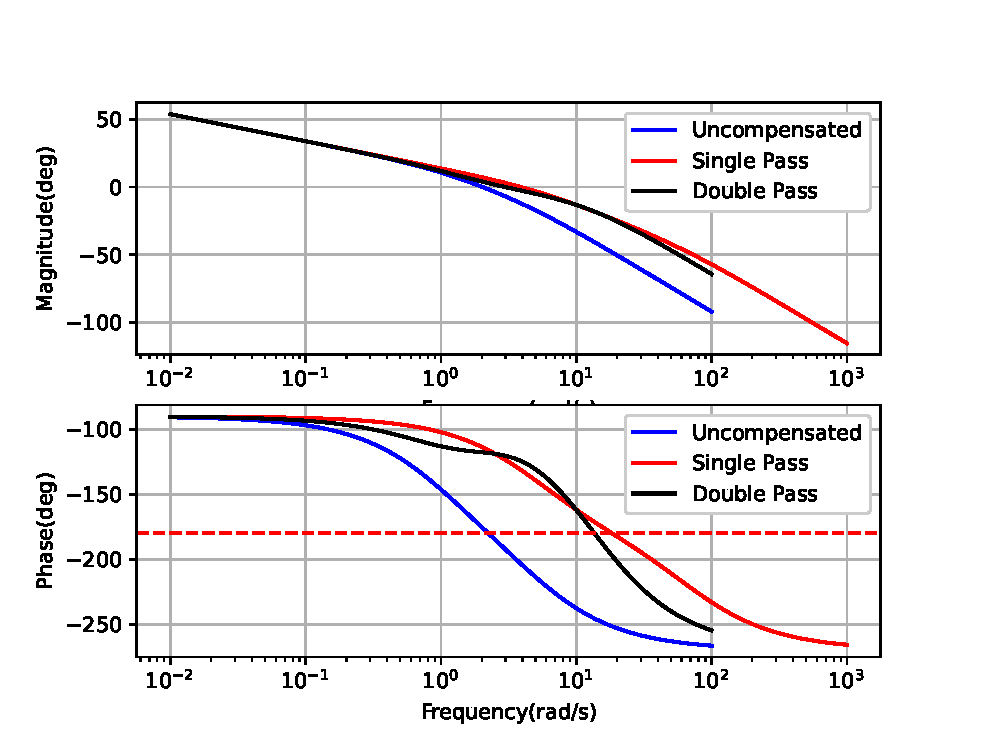
\includegraphics[width=\columnwidth]{./figs/ee18btech11051/ee18btech11051_fig3.eps}
    \label{fig:ee18btech11051_3}
\end{figure}

\\

\begin{table}[!ht]
\centering
%%%%%%%%%%%%%%%%%%%%%%%%%%%%%%%%%%%%%%%%%%%%%%%%%%%%%%%%%%%%%%%%%%%%%%
%%                                                                  %%
%%  This is the header of a LaTeX2e file exported from Gnumeric.    %%
%%                                                                  %%
%%  This file can be compiled as it stands or included in another   %%
%%  LaTeX document. The table is based on the longtable package so  %%
%%  the longtable options (headers, footers...) can be set in the   %%
%%  preamble section below (see PRAMBLE).                           %%
%%                                                                  %%
%%  To include the file in another, the following two lines must be %%
%%  in the including file:                                          %%
%%        \def\inputGnumericTable{}                                 %%
%%  at the beginning of the file and:                               %%
%%        \input{name-of-this-file.tex}                             %%
%%  where the table is to be placed. Note also that the including   %%
%%  file must use the following packages for the table to be        %%
%%  rendered correctly:                                             %%
%%    \usepackage[latin1]{inputenc}                                 %%
%%    \usepackage{color}                                            %%
%%    \usepackage{array}                                            %%
%%    \usepackage{longtable}                                        %%
%%    \usepackage{calc}                                             %%
%%    \usepackage{multirow}                                         %%
%%    \usepackage{hhline}                                           %%
%%    \usepackage{ifthen}                                           %%
%%  optionally (for landscape tables embedded in another document): %%
%%    \usepackage{lscape}                                           %%
%%                                                                  %%
%%%%%%%%%%%%%%%%%%%%%%%%%%%%%%%%%%%%%%%%%%%%%%%%%%%%%%%%%%%%%%%%%%%%%%



%%  This section checks if we are begin input into another file or  %%
%%  the file will be compiled alone. First use a macro taken from   %%
%%  the TeXbook ex 7.7 (suggestion of Han-Wen Nienhuys).            %%
\def\ifundefined#1{\expandafter\ifx\csname#1\endcsname\relax}


%%  Check for the \def token for inputed files. If it is not        %%
%%  defined, the file will be processed as a standalone and the     %%
%%  preamble will be used.                                          %%
\ifundefined{inputGnumericTable}

%%  We must be able to close or not the document at the end.        %%
	\def\gnumericTableEnd{\end{document}}


%%%%%%%%%%%%%%%%%%%%%%%%%%%%%%%%%%%%%%%%%%%%%%%%%%%%%%%%%%%%%%%%%%%%%%
%%                                                                  %%
%%  This is the PREAMBLE. Change these values to get the right      %%
%%  paper size and other niceties.                                  %%
%%                                                                  %%
%%%%%%%%%%%%%%%%%%%%%%%%%%%%%%%%%%%%%%%%%%%%%%%%%%%%%%%%%%%%%%%%%%%%%%

	\documentclass[12pt%
			  %,landscape%
                    ]{report}
       \usepackage[latin1]{inputenc}
       \usepackage{fullpage}
       \usepackage{color}
       \usepackage{array}
       \usepackage{longtable}
       \usepackage{calc}
       \usepackage{multirow}
       \usepackage{hhline}
       \usepackage{ifthen}

	\begin{document}


%%  End of the preamble for the standalone. The next section is for %%
%%  documents which are included into other LaTeX2e files.          %%
\else

%%  We are not a stand alone document. For a regular table, we will %%
%%  have no preamble and only define the closing to mean nothing.   %%
    \def\gnumericTableEnd{}

%%  If we want landscape mode in an embedded document, comment out  %%
%%  the line above and uncomment the two below. The table will      %%
%%  begin on a new page and run in landscape mode.                  %%
%       \def\gnumericTableEnd{\end{landscape}}
%       \begin{landscape}


%%  End of the else clause for this file being \input.              %%
\fi

%%%%%%%%%%%%%%%%%%%%%%%%%%%%%%%%%%%%%%%%%%%%%%%%%%%%%%%%%%%%%%%%%%%%%%
%%                                                                  %%
%%  The rest is the gnumeric table, except for the closing          %%
%%  statement. Changes below will alter the table's appearance.     %%
%%                                                                  %%
%%%%%%%%%%%%%%%%%%%%%%%%%%%%%%%%%%%%%%%%%%%%%%%%%%%%%%%%%%%%%%%%%%%%%%

\providecommand{\gnumericmathit}[1]{#1} 
%%  Uncomment the next line if you would like your numbers to be in %%
%%  italics if they are italizised in the gnumeric table.           %%
%\renewcommand{\gnumericmathit}[1]{\mathit{#1}}
\providecommand{\gnumericPB}[1]%
{\let\gnumericTemp=\\#1\let\\=\gnumericTemp\hspace{0pt}}
 \ifundefined{gnumericTableWidthDefined}
        \newlength{\gnumericTableWidth}
        \newlength{\gnumericTableWidthComplete}
        \newlength{\gnumericMultiRowLength}
        \global\def\gnumericTableWidthDefined{}
 \fi
%% The following setting protects this code from babel shorthands.  %%
 \ifthenelse{\isundefined{\languageshorthands}}{}{\languageshorthands{english}}
%%  The default table format retains the relative column widths of  %%
%%  gnumeric. They can easily be changed to c, r or l. In that case %%
%%  you may want to comment out the next line and uncomment the one %%
%%  thereafter                                                      %%
\providecommand\gnumbox{\makebox[0pt]}
%%\providecommand\gnumbox[1][]{\makebox}

%% to adjust positions in multirow situations                       %%
\setlength{\bigstrutjot}{\jot}
\setlength{\extrarowheight}{\doublerulesep}

%%  The \setlongtables command keeps column widths the same across  %%
%%  pages. Simply comment out next line for varying column widths.  %%
\setlongtables

\setlength\gnumericTableWidth{%
	80pt+%
	50pt+%
	60pt+%
0pt}
\def\gumericNumCols{3}
\setlength\gnumericTableWidthComplete{\gnumericTableWidth+%
         \tabcolsep*\gumericNumCols*2+\arrayrulewidth*\gumericNumCols}
\ifthenelse{\lengthtest{\gnumericTableWidthComplete > \linewidth}}%
         {\def\gnumericScale{\ratio{\linewidth-%
                        \tabcolsep*\gumericNumCols*2-%
                        \arrayrulewidth*\gumericNumCols}%
{\gnumericTableWidth}}}%
{\def\gnumericScale{1}}

%%%%%%%%%%%%%%%%%%%%%%%%%%%%%%%%%%%%%%%%%%%%%%%%%%%%%%%%%%%%%%%%%%%%%%
%%                                                                  %%
%% The following are the widths of the various columns. We are      %%
%% defining them here because then they are easier to change.       %%
%% Depending on the cell formats we may use them more than once.    %%
%%                                                                  %%
%%%%%%%%%%%%%%%%%%%%%%%%%%%%%%%%%%%%%%%%%%%%%%%%%%%%%%%%%%%%%%%%%%%%%%

\ifthenelse{\isundefined{\gnumericColA}}{\newlength{\gnumericColA}}{}\settowidth{\gnumericColA}{\begin{tabular}{@{}p{80pt*\gnumericScale}@{}}x\end{tabular}}

\ifthenelse{\isundefined{\gnumericColB}}{\newlength{\gnumericColB}}{}\settowidth{\gnumericColB}{\begin{tabular}{@{}p{50pt*\gnumericScale}@{}}x\end{tabular}}

\ifthenelse{\isundefined{\gnumericColC}}{\newlength{\gnumericColC}}{}\settowidth{\gnumericColC}{\begin{tabular}{@{}p{60pt*\gnumericScale}@{}}x\end{tabular}}
\begin{tabular}[c]{%
	b{\gnumericColA}%	
	b{\gnumericColB}%
	b{\gnumericColC}%
	}

%%%%%%%%%%%%%%%%%%%%%%%%%%%%%%%%%%%%%%%%%%%%%%%%%%%%%%%%%%%%%%%%%%%%%%
%%  The longtable options. (Caption, headers... see Goosens, p.124) %%
%	\caption{The Table Caption.}             \\	%
% \hline	% Across the top of the table.
%%  The rest of these options are table rows which are placed on    %%
%%  the first, last or every page. Use \multicolumn if you want.    %%

%%  Header for the first page.                                      %%
%	\multicolumn{3}{c}{The First Header} \\ \hline 
%	\multicolumn{1}{c}{colTag}	%Column 1
%	&\multicolumn{1}{c}{colTag}	%Column 2
%	&\multicolumn{1}{c}{colTag}	\\ \hline %Last column
%	\endfirsthead

%%  The running header definition.                                  %%
%	\hline
%	\multicolumn{3}{l}{\ldots\small\slshape continued} \\ \hline
%	\multicolumn{1}{c}{colTag}	%Column 1
%	&\multicolumn{1}{c}{colTag}	%Column 2
%	&\multicolumn{1}{c}{colTag}	\\ \hline %Last column
%	\endhead

%%  The running footer definition.                                  %%
%	\hline
%	\multicolumn{3}{r}{\small\slshape continued\ldots} \\
%	\endfoot

%%  The ending footer definition.                                   %%
%	\multicolumn{3}{c}{That's all folks} \\ \hline 
%	\endlastfoot
%%%%%%%%%%%%%%%%%%%%%%%%%%%%%%%%%%%%%%%%%%%%%%%%%%%%%%%%%%%%%%%%%%%%%%


	
\hhline{---}
	 \multicolumn{1}{|p{\gnumericColA}|}%
	{\gnumericPB{\centering}\textbf{Parameter}}
	&\multicolumn{1}{p{\gnumericColB}|}%
	{\gnumericPB{\centering}\textbf{Expected}}
	&\multicolumn{1}{p{\gnumericColC}|}%
	{\gnumericPB{\centering}\textbf{Final}}

\\

	

\hhline{|---|}
	 \multicolumn{1}{|p{\gnumericColA}|}%
	{\gnumericPB{\centering}Phase Margin}
	&\multicolumn{1}{p{\gnumericColB}|}%
	{\gnumericPB{\centering}$60^{\degree}$}
	&\multicolumn{1}{p{\gnumericColC}|}%
	{\gnumericPB{\centering}$59.68^{\degree}$}
	
	



\\


\hhline{|---|}
	 \multicolumn{1}{|p{\gnumericColA}|}%
	{\gnumericPB{\centering}$K_{v}$}
	&\multicolumn{1}{p{\gnumericColB}|}%
	{\gnumericPB{\centering}$5$}
	&\multicolumn{1}{p{\gnumericColC}|}%
	{\gnumericPB{\centering} $5$}

\\


\hhline{|---|}
	 \multicolumn{1}{|p{\gnumericColA}|}%
	{\gnumericPB{\centering}$\omega_{gc}$}
	&\multicolumn{1}{p{\gnumericColB}|}%
	{\gnumericPB{\centering}$>=2.03$}
	&\multicolumn{1}{p{\gnumericColC}|}%
	{\gnumericPB{\centering} $3.01$}

\\

\hhline{|-|-|-}
\end{tabular}

\ifthenelse{\isundefined{\languageshorthands}}{}{\languageshorthands{\languagename}}
\gnumericTableEnd

\caption{Table of Specifications}
\label{table:ee18btech11026_table_1}
\end{table}
\\~\\

As it can be seen from the final readings in the table \ref{table:ee18btech11026_table_1}, the desired transfer function is achieved. 

\end{enumerate}
